%\documentclass{beamer}
\documentclass[9pt, table]{beamer}

\usepackage[slovene]{babel}
\usepackage{amsfonts,amssymb}
\usepackage[utf8]{inputenc}
\usepackage{lmodern}
\usepackage[T1]{fontenc}

\usepackage{mathptmx}
\usepackage{helvet}
\usepackage{courier}

\setbeamercovered{transparent}

\usetheme{Warsaw}
\usecolortheme{rose}

\newtheorem{izrek}{Izrek}
\newtheorem{definicija}{Definicija}
\newtheorem{primer}{Primer}
\newtheorem{trditev}{Trditev}
\newtheorem{oznaka}{Oznaka}

\newcommand{\R}{\mathbb R}
\newcommand{\N}{\mathbb N}
\newcommand{\Z}{\mathbb Z}
\newcommand{\C}{\mathbb C}
\newcommand{\Q}{\mathbb Q}

\newcommand{\pojem}[1]{\textsc{#1}}


\title{Minimalne ploskve}
\author{Tjaša Vrhovnik}

\institute{Mentor: prof.~dr.~Franc Forstnerič\\
	Univerza v Ljubljani\\
	Fakulteta za matematiko in fiziko\\
	Oddelek za matematiko}
\date{10.\ maj 2020}

\begin{document}

%%%%%%%%%%%%%%%%%%%%%%%%%%%%%%%%%%%%%%%%%%%

\begin{frame}
\titlepage
\end{frame}

%%%%%%%%%%%%%%%%%%%%%%%%%%%%%%%%%%%%%%%%%%%

\begin{frame}
\frametitle{Načrt}

\begin{enumerate}
\item Motivacija
\item Osnovne definicije
\item Minimalne ploskve
\item Aproksimacija minimalnih ploskev
\item Primeri
\end{enumerate}

\end{frame}

%%%%%%%%%%%%%%%%%%%%%%%%%%%%%%%%%%%%%%%%%%%

\begin{frame}
\frametitle{Motivacija}

\begin{itemize}
\item ploskve z lokalno minimalno ploščino
\item Euler, Lagrange, Meusnier (18. st.)
\item Plateaujev problem
\item Riemannove ploskve
\end{itemize}

\begin{center}
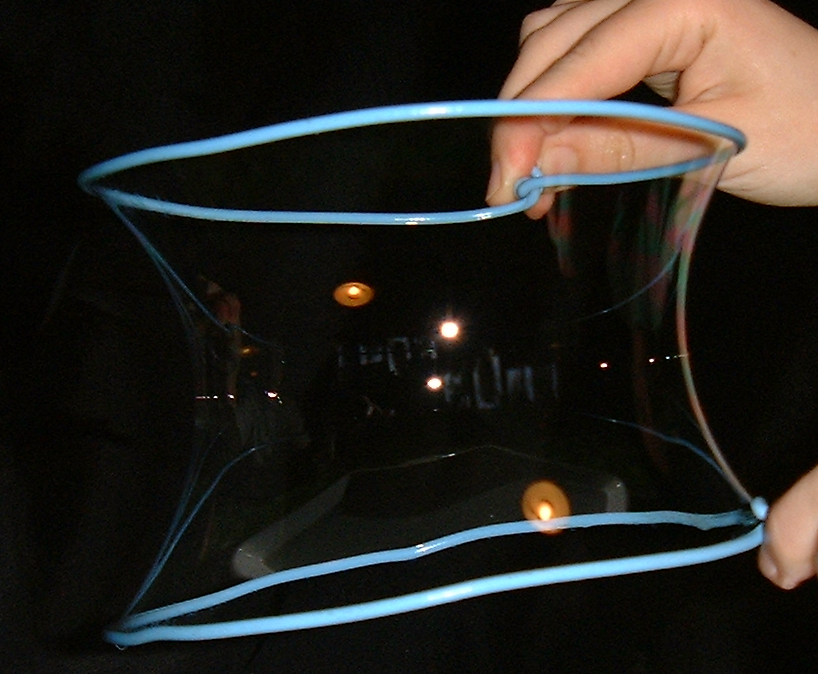
\includegraphics[scale=0.18]{milni-mehurcek.png}
\end{center}

\end{frame}

%%%%%%%%%%%%%%%%%%%%%%%%%%%%%%%%%%%%%%%%%%%

\begin{frame}
\frametitle{Osnovne definicije}

\begin{definicija}
Naj bo $n \in \N_{0}$. Topološki prostor $M$ z lastnostmi:
\begin{enumerate}
\item $M$ je Hausdorffov,
\item $M$ je 2-števen,
\item $M$ je lokalno evklidski prostor dimenzije $n$ (za vsak $x \in M$ obstajata odprta okolica $U \subset M$ in homeomorfizem $\phi \colon U \to \phi(U) \subset \R^{n}$, kjer je $\phi(U)$ odprta množica),
\end{enumerate}
imenujemo \textup{topološka mnogoterost} dimenzije $n$.
\end{definicija}

\pause
\begin{definicija}
\textup{Riemannova ploskev} je kompleksna mnogoterost kompleksne dimenzije $1$.
\end{definicija}

\end{frame}

%%%%%%%%%%%%%%%%%%%%%%%%%%%%%%%%%%%%%%%%%%%

\begin{frame}
\frametitle{Osnovne definicije}

\begin{definicija}
Naj bo $f \colon M \to N$ gladka preslikava med gladkima mnogoterostima. Preslikava $f$ se imenuje \textup{imerzija}, če je njen diferencial $df_{x}$ injektiven v vsaki točki $x \in M$.
\end{definicija}

\pause
Na prostoru $\R^{n}$ s koordinatami $x = (x_{1}, \dots, x_{n})$ je definirana \emph{Evklidska metrika}
\begin{equation}
ds^2 = (dx_{1})^2 + \cdots + (dx_{n})^2.
\end{equation}
Naj bo $D$ domena v $\R^2$ in $x \colon D \to \R^{n}$ imerzija, podana s predpisom $x(u_1,u_2) = (x_{1}(u_1,u_2), \dots, x_{n}(u_1,u_2))$, $(u_1,u_2) \in D$. Pripadajoča metrika na $D$ je enaka
\begin{gather}
g = x^{*}ds^2 = g_{1,1}du_{1}^2 + g_{1,2}du_{1}du_{2} + g_{2,1}du_{2}du_{1} + g_{2,2}du_{2}^2, \\
g_{1,1} = |x_{u_1}|^2, \ g_{1,2} = g_{2,1} = x_{u_1} \cdot x_{u_2}, \ g_{2,2} = |x_{u_2}|^2.
\end{gather}

\end{frame}

%%%%%%%%%%%%%%%%%%%%%%%%%%%%%%%%%%%%%%%%%%%

\begin{frame}
\frametitle{Osnovne definicije}

\begin{definicija}
\begin{enumerate}
\item
Naj bo $M$ gladka kompaktna ploskev z robom, $n \geq 3$ in naj bo preslikava $x \colon M \to \R^{n}$ imerzija razreda $\mathcal{C}^2$. \textup{Variacija preslikave x s fiksnim robom} je 1-parametrična družina $\mathcal{C}^2$ preslikav 
\begin{gather}
x^{t} \colon M \to \R^{n},\ t \in (-\varepsilon, \varepsilon) \subset \R,
\end{gather}
če je $x^0 = x$ in za vse $t$ z intervala velja $x^{t} = x$ na $bM$.
%
\item
Naj bo $p \in M$. \textup{Variacijsko vektorsko polje} preslikave $x^{t}$ je vektorsko polje, definirano kot
\begin{equation}
E(p,t) = \frac{\partial{x^t(p)}}{\partial{t}} \in \R^{n}.
\end{equation}
\end{enumerate}
\end{definicija}

\end{frame}

%%%%%%%%%%%%%%%%%%%%%%%%%%%%%%%%%%%%%%%%%%%

\begin{frame}
\frametitle{Minimalne ploskve}

\begin{definicija}
Naj bo $x \colon M \to \R^{n}$ imerzija razreda $\mathcal{C}^2$. Sliko $x(M)$ imenujemo \textup{minimalna ploskev}, če za vsako kompaktno domeno $D \subset M$ z gladkim robom $bD$ in vsako gladko variacijo $x^{t}$ preslikave $x$ s fiksnim robom velja
\begin{equation} \label{eq:1-var-ploščine}
\frac{d}{dt} \Big|_{t=0} \text{Area}(x^{t}(D)) = 0.
\end{equation}
Ekvivalentno pravimo, da je minimalna ploskev stacionarna točka ploskovnega funkcionala $\text{Area}$.
\end{definicija}

\end{frame}

%%%%%%%%%%%%%%%%%%%%%%%%%%%%%%%%%%%%%%%%%%%

\begin{frame}
\frametitle{Minimalne ploskve}

\begin{izrek}[Prva variacijska formula] \label{izr:1-var-formula}
Naj bo $M$ gladka kompaktna ploskev z robom, $n \geq 3$ in $x \colon M \to \R^{n}$ imerzija razreda $\mathcal{C}^2$. Naj bo $E = \partial{x^{t}} / \partial{t}|_{t=0}$ variacijsko vektorsko polje preslikave $x^{t}$ pri $t=0$, $\textbf{\textup{H}}$ vektorsko polje povprečne ukrivljenosti preslikave $x$ in $dA$ ploščinski element glede na Riemannovo metriko $x^{*}ds^2$, definirano na $M$.
Potem za vsako gladko variacijo $x^{t} \colon M \to \R^{n}$ imerzije $x$ s fiksnim robom velja
\begin{equation} \label{eq:1-var-formula}
\frac{d}{dt} \Big|_{t=0} \text{Area}(x^{t}(M)) = -2 \int_{M} {E \cdot \textbf{\textup{H}} dA}.
\end{equation}
\end{izrek}

\end{frame}

%%%%%%%%%%%%%%%%%%%%%%%%%%%%%%%%%%%%%%%%%%%

\begin{frame}
\frametitle{Minimalne ploskve}

\begin{izrek}
Naj bo $M$ odprta Riemannova ploskev, $n \geq 3$ in $x = (x_1, \dots , x_n) \colon M \to \R^{n}$ konformna imerzija razreda $\mathcal{C}^2$. Ekvivalentno je:
\begin{enumerate}
	\item $x$ je minimalna ploskev.
	\item Vektorsko polje povprečne ukrivljenosti preslikave $x$ je ničelno.
	\item $x$ je harmonična.
	\item 1-forma $ \partial{x} = (\partial{x_1}, \dots , \partial{x_n})$ z vrednostmi v $\C^{n}$ je holomorfna in velja
			\begin{equation}
			(\partial{x_1})^2 + \cdots + (\partial{x_n})^2 = 0.
			\end{equation}
	\item Naj bo $\theta$ holomorfna 1-forma na $M$, ki ni nikjer enaka $0$. Potem je preslikava $f = 2\partial{x} / \theta \colon M \to \C^{n}$ holomorfna z 				vrednostmi v \emph{ničelni kvadriki}
			\begin{equation} \label{ničelna-kvadrika}		
			\textbf{\textup{A}} = \{ (z_1, \dots , z_n) \in \C^{n} ; \ z_{1}^{2} + \cdots + z_{n}^{2} = 0 \}.
			\end{equation}	
		Nadalje je Riemannova metrika na $M$, inducirana s konformno imerzijo $x$, enaka
			\begin{align}
			g &= x^{*} ds^2 = |dx_1|^2 + \cdots + |dx_n|^2 = 2 (|\partial{x_1}|^2 + \cdots |\partial{x_n}|^2).
			\end{align}			
\end{enumerate}
\end{izrek}

\end{frame}

%%%%%%%%%%%%%%%%%%%%%%%%%%%%%%%%%%%%%%%%%%%

\begin{frame}
\frametitle{Minimalne ploskve}

\begin{izrek}[Weierstrassova predstavitev konformnih minimalnih ploskev]
Naj bo $n \geq 3$ in $M$ odprta Riemannova ploskev, na kateri definiramo holomorfno 1-formo $\phi = (\phi_{1}, \dots , \phi_{n})$ z vrednostmi v $\C^{n}$, ki je povsod neničelna, in zadošča 
\begin{enumerate}
\item $ \sum_{j=1}^{n} \phi_{j}^{2} = 0$,
\item $ \Re \int_{C} \phi = 0 $ za vse $[C] \in H_{1} (M, \Z)$.
\end{enumerate}
Potem za poljuben izbor točk $p_0 \in M$ in $x_0 \in \R^{n}$ predpis $x \colon M \to \R^{n}$,
\begin{align} \label{eq:Wstrass-kmi}
x(p) = x_0 + \Re \int_{p_0}^{p} \phi, \ p \in M,
\end{align}
podaja dobro definirano konformno minimalno imerzijo. Zanjo velja
\begin{align}
2 \partial{x} = \phi \quad \text{in} \quad g = x^{*} ds^2 = |dx|^2 = \frac{1}{2} |\phi|^2.
\end{align}
\end{izrek}

\end{frame}

%%%%%%%%%%%%%%%%%%%%%%%%%%%%%%%%%%%%%%%%%%%

\begin{frame}
\frametitle{Izreki o aproksimaciji in interpolaciji}

\begin{definicija}
Naj bo $M$ gladka ploskev, $K$ končna unija paroma disjunktnih kompaktnih domen s kosoma zvezno odvedljivimi robovi v $M$ ter $E = S \setminus K^\circ$ unija končno mnogo paroma disjunktnih gladkih Jordanovih lokov in zaprtih Jordanovih krivulj, ki se dotikajo $K$ kvečjemu v svojih krajiščih in sekajo rob $K$ transverzalno. Kompaktno podmnožico v $M$ oblike $S = K \cup E$ imenujemo \textup{dopustna množica}.
\end{definicija}

\pause
\begin{definicija}
Naj bo $x \colon M \to \R^{n}$ harmonična preslikava. Njen \textup{pretok} je homomorfizem grup $\textup{Flux}_{x} \colon H_{1} (M, \Z) \to \R^{n}$, definiran s predpisom 
\begin{equation}
\textup{Flux}_{x} ([C]) = \int_{C} {d^{c} x}.
\end{equation}
\end{definicija}

\end{frame}

%%%%%%%%%%%%%%%%%%%%%%%%%%%%%%%%%%%%%%%%%%%

\begin{frame}
\frametitle{Izreki o aproksimaciji in interpolaciji}

\begin{definicija}
Naj bo $S = K \cup E$ dopustna podmnožica Riemannove ploskve $M$ in $\theta$ povsod neničelna holomorfna 1-forma, definirana v okolici $S \subset M$.
Naj bosta $n \geq 3$ in $r \in \N$. \textup{Posplošena konformna minimalna imerzija} $S \to \R^{n}$ razreda $\mathcal{C}^{r}$ je par $(x, f \theta)$, kjer je $x \colon S \to \R^{n}$ preslikava razreda  $\mathcal{C}^{r}$, njena zožitev na $S^\circ = K^\circ$ je konformna minimalna imerzija in preslikava $f \in \mathcal{A}^{r-1}(S, \textbf{\textup{A}}_{*})$ zadošča naslednjima pogojema:
\begin{enumerate}
\item na množici $K$ velja $f \theta = 2 \partial x$;
\item za vsako gladko pot $\alpha$ v $M$, ki parametrizira povezano komponento $E = \overline{S \setminus K}$ velja $ \Re(\alpha^{*}(f \theta)) = \alpha^{*}(dx) = d(x \circ \alpha)$.
\end{enumerate}
\end{definicija}

\end{frame}

%%%%%%%%%%%%%%%%%%%%%%%%%%%%%%%%%%%%%%%%%%%

\begin{frame}
\frametitle{Izreki o aproksimaciji in interpolaciji}
 
\begin{izrek} [Bishop-Mergelyanov aproksimacijski izrek] \label{izr:Bishop-Mergelyan}
Naj bo $M$ odprta Riemannova ploskev in $K$ njena kompaktna podmnožica brez lukenj ($K$ je Rungejeva v $M$). Potem lahko vsako funkcijo v $\mathcal{A}(K)$ aproksimiramo enakomerno na $K$ s funkcijami v $\mathcal{O}(M)$.
\end{izrek}

\begin{izrek} [Weierstrass-Florackov interpolacijski izrek]
Naj bo $M$ odprta Riemannova ploskev in $K$ njena Rungejeva podmnožica. Naj bo $A = \{ a_i \}_{i=1}^{\infty}$ zaprta diskretna podmnožica v $M$, $U$ odprta podmnožica $M$, tako da je $A \cup K \subset U$ in $f$ meromorfna funkcija na $U$ z ničlami in poli le v točkah množice $A$.
Potem za izbrane $\varepsilon > 0$ in števila $k_{i} \in \N$ obstaja meromorfna funkcija $F$ na $M$, za katero velja:
\begin{enumerate}
\item $|F(z) - f(z)| < \varepsilon$ za vse $z \in K$,
\item v točkah $a_i$ je razlika $F-f$ ničelna do reda $k_i$,
\item $F$ nima ničel in polov na $M \backslash A$.
\end{enumerate} 
\end{izrek}

\end{frame}

%%%%%%%%%%%%%%%%%%%%%%%%%%%%%%%%%%%%%%%%%%%

\begin{frame}
\frametitle{Aproksimacija minimalnih ploskev}

\begin{trditev}
Naj bo $M$ odprta Riemannova ploskev in $\theta$ povsod neničelna holomorfna 1-forma na $M$.
Naj bo $S$ povezana dopustna množica, ki je Rungejeva v $M$, in $A=\{a_{1}, \dots , a_{k} \} \subset S$. Naj bosta $r, s \in \N$. 

Potem lahko vsako posplošeno konformno minimalno imerzijo $(x, f\theta) \in GCMI^{r}(S,\R^{n})$ aproksimiramo s konformnimi minimalnimi imerzijami $X \colon M \to \R^{n}$ razreda $\mathcal{C}^{r}$, za katere velja $\textup{Flux}_{X} = \textup{Flux}_{x}$. 
\end{trditev}

\end{frame}

%%%%%%%%%%%%%%%%%%%%%%%%%%%%%%%%%%%%%%%%%%%

\begin{frame}
\frametitle{Aproksimacija minimalnih ploskev}

\begin{izrek}[Mergelyanov izrek za konformne minimalne ploskve]
Naj bo $M$ odprta Riemannova ploskev, $\theta$ povsod neničelna holomorfna 1-forma na $M$, $n \geq 3$ in $r \geq 1$.
Naj bo $S$ dopustna Rungejeva množica v $M$ in $A$ zaprta diskretna podmnožica $M$. 
Naj bo $x \colon S \to \R^{n}$ posplošena konformna minimalna imerzija razreda $\mathcal{C}^{r}(S, \R^{n})$, ki je konformna minimalna imerzija v okolici vsake točke iz $A$.

Za izbrane $\varepsilon > 0$, preslikavo $k \colon A \to \N$ in homomorfizem grup $\mathfrak{p} \colon H_{1}(M,\Z) \to \R^{n}$, $\mathfrak{p}|_{H_{1}(S,\Z)} = \textup{Flux}_{x}$, obstaja konformna minimalna imerzija $\tilde{x} \colon M \to \R^{n}$, za katero velja:
\begin{enumerate}
\item $||\tilde{x} - x||_{\mathcal{C}^{r}(S)} < \varepsilon$.
\item Razlika $\tilde{x}-x$ je ničelna do reda $k(p)$ v vsaki točki $p\in A$.
\item $Flux_{\tilde{x}} = \mathfrak{p}$ na $H_{1}(M,\Z)$.
\item Če je $n\geq5$ in je $x \colon A \to \R^{n}$ injektivna preslikava, potem je $\tilde{x}$ injektivna imerzija.
\item Če je $n=4$ in ima $x$ enostavne dvojne točke na množici $A$, potem je $\tilde{x}$ imerzija z enostavnimi dvojnimi točkami na $A$.
\end{enumerate}
\end{izrek}

\end{frame}

%%%%%%%%%%%%%%%%%%%%%%%%%%%%%%%%%%%%%%%%%%%

\begin{frame}
\frametitle{Primeri}

KATENOIDA
\begin{align*}
x &\colon \R^{2} \to \R^{3} \\
x(u,v) &= (\cos u \cdot \cosh v, \sin u \cdot \cosh v, v)
\end{align*}
%
\begin{center}
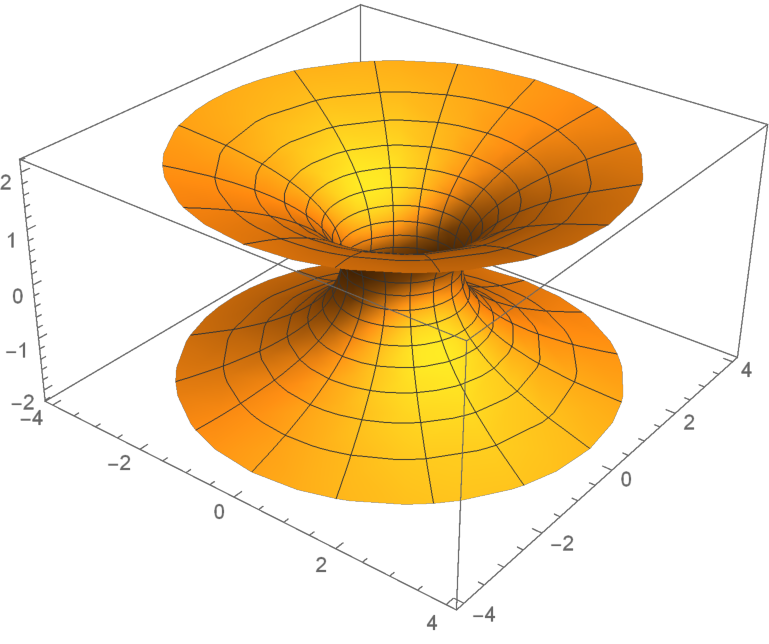
\includegraphics[scale=0.5]{catenoid.pdf}
\end{center}

\end{frame}

%%%%%%%%%%%%%%%%%%%%%%%%%%%%%%%%%%%%%%%%%%%

\begin{frame}
\frametitle{Primeri}

HELIKOID
\begin{align*}
x &\colon \R^{2} \to \R^{3} \\
x(u,v) &= (\sin u \cdot \sinh v, -\cos u \cdot \sinh v, u)
\end{align*}
%
\begin{center}
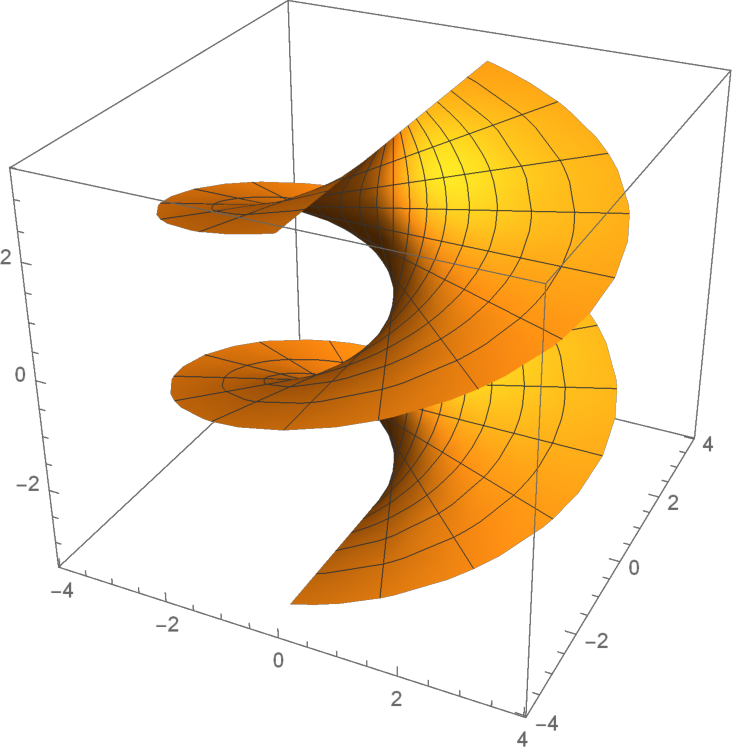
\includegraphics[scale=0.4]{helicoid.pdf}
\end{center}

\end{frame}

%%%%%%%%%%%%%%%%%%%%%%%%%%%%%%%%%%%%%%%%%%%

\begin{frame}
\frametitle{Primeri}


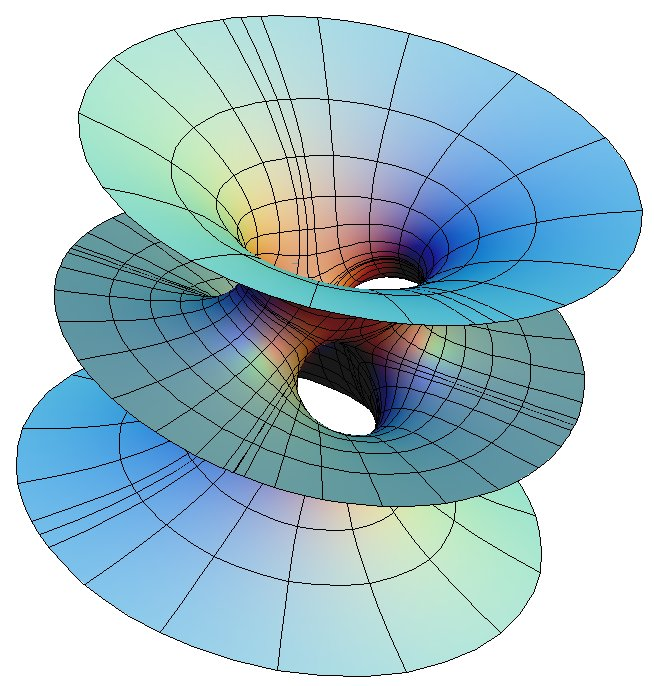
\includegraphics[scale=0.2]{costa.jpg}
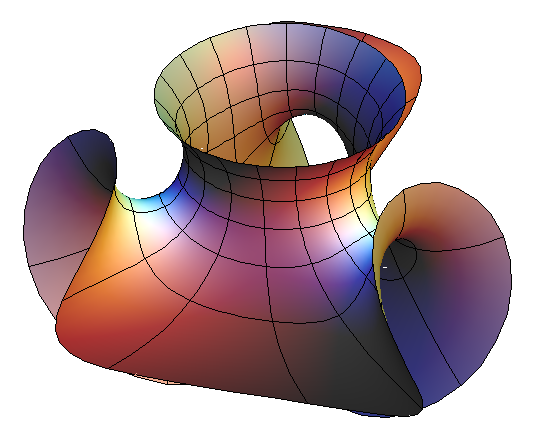
\includegraphics[scale=0.3]{catenoid-enneper.png}


\end{frame}

\end{document}